%% Tex spellcheck = fr_FR
\addcontentsline{toc}{chapter}{appendixs} % Adding toc entry
%%% COMMENT THESES LINES IF YOU DO NOT USE DEDICATED TOC FOR appendixS
\stopcontents[default]
\resumecontents[annexes]
%%% /COMMENT THESES LINES IF YOU DO NOT USE DEDICATED TOC FOR ANNEXES
\chapter*{appendixs}

\chapter*{appendix 1}
\addcontentsline{toc}{chapter}{appendix 1}

% Simple centered unnumbered title
\begin{center}
	\textbf{Gnu Radio Configuration for position fix on raw data}
	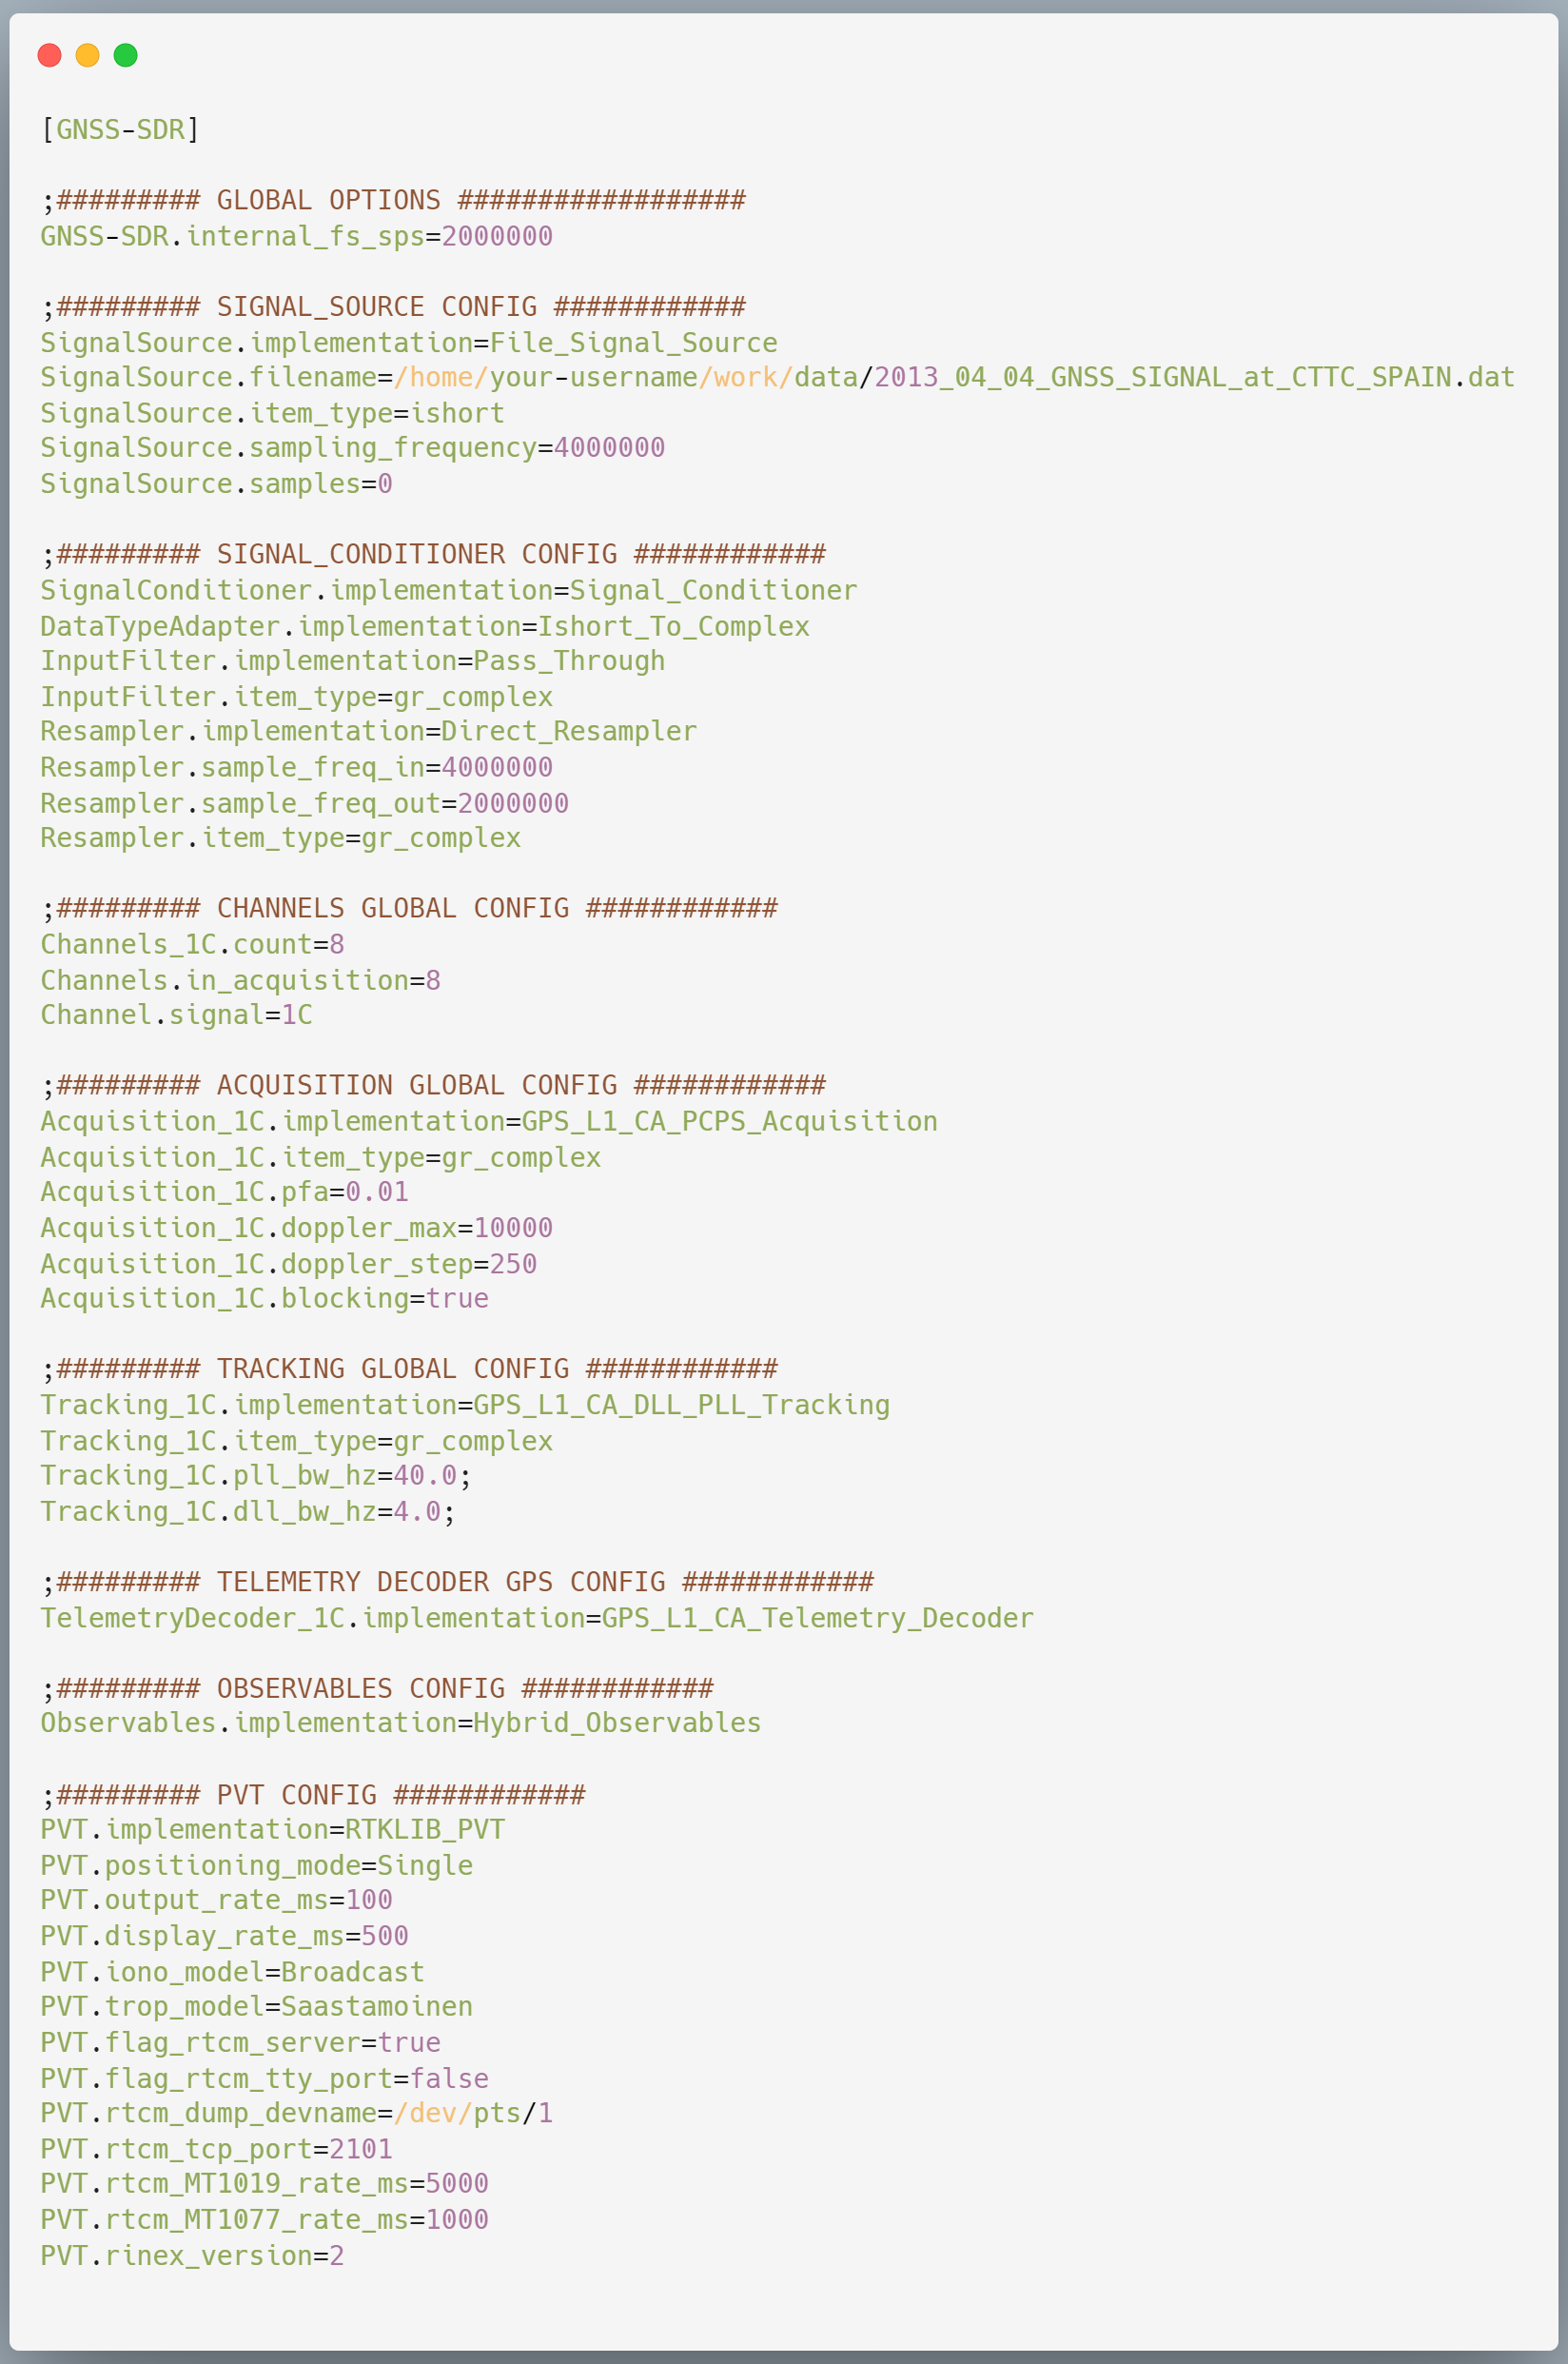
\includegraphics[width=0.8\linewidth]{config_gnu_radio.png}
\end{center}


\chapter*{appendix 2}
\addcontentsline{toc}{chapter}{appendix 2}
\begin{center}
	\textbf{GNSS Sdr configuration for USRP B200 as frontend}
\end{center}
\begin{center}
	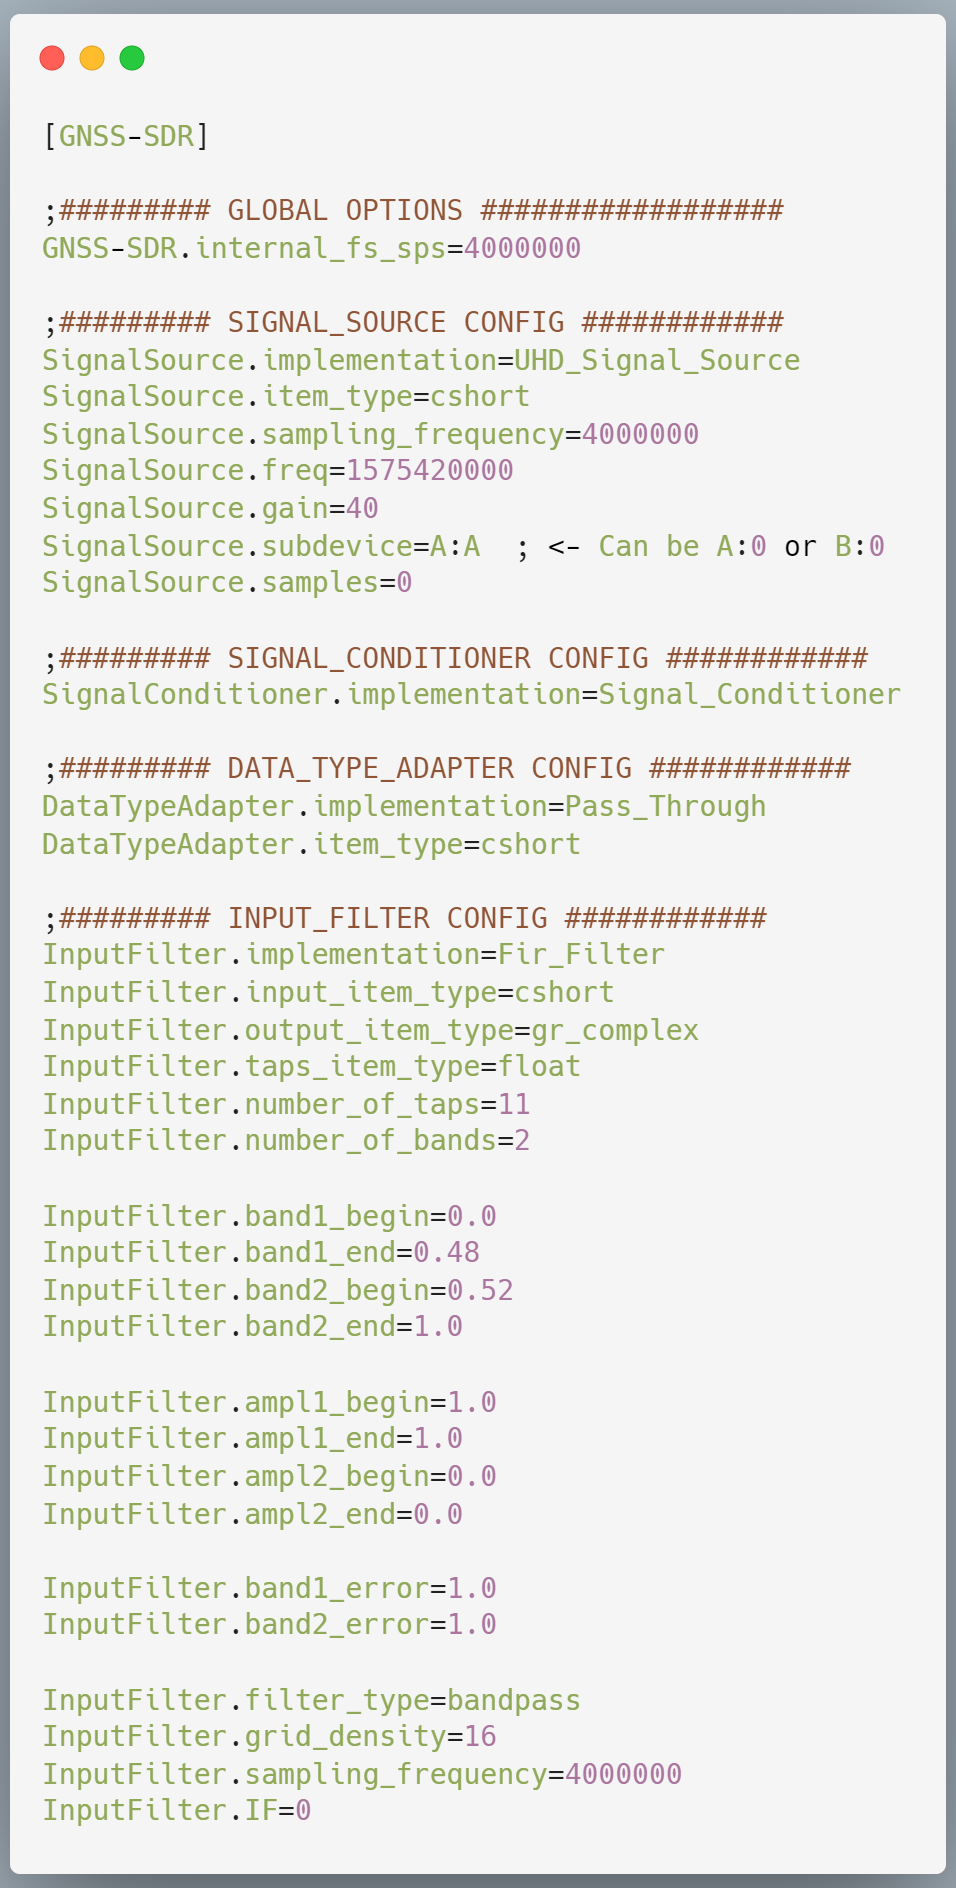
\includegraphics[width=0.6\linewidth]{sdr_front.png}
\end{center}
\begin{center}
	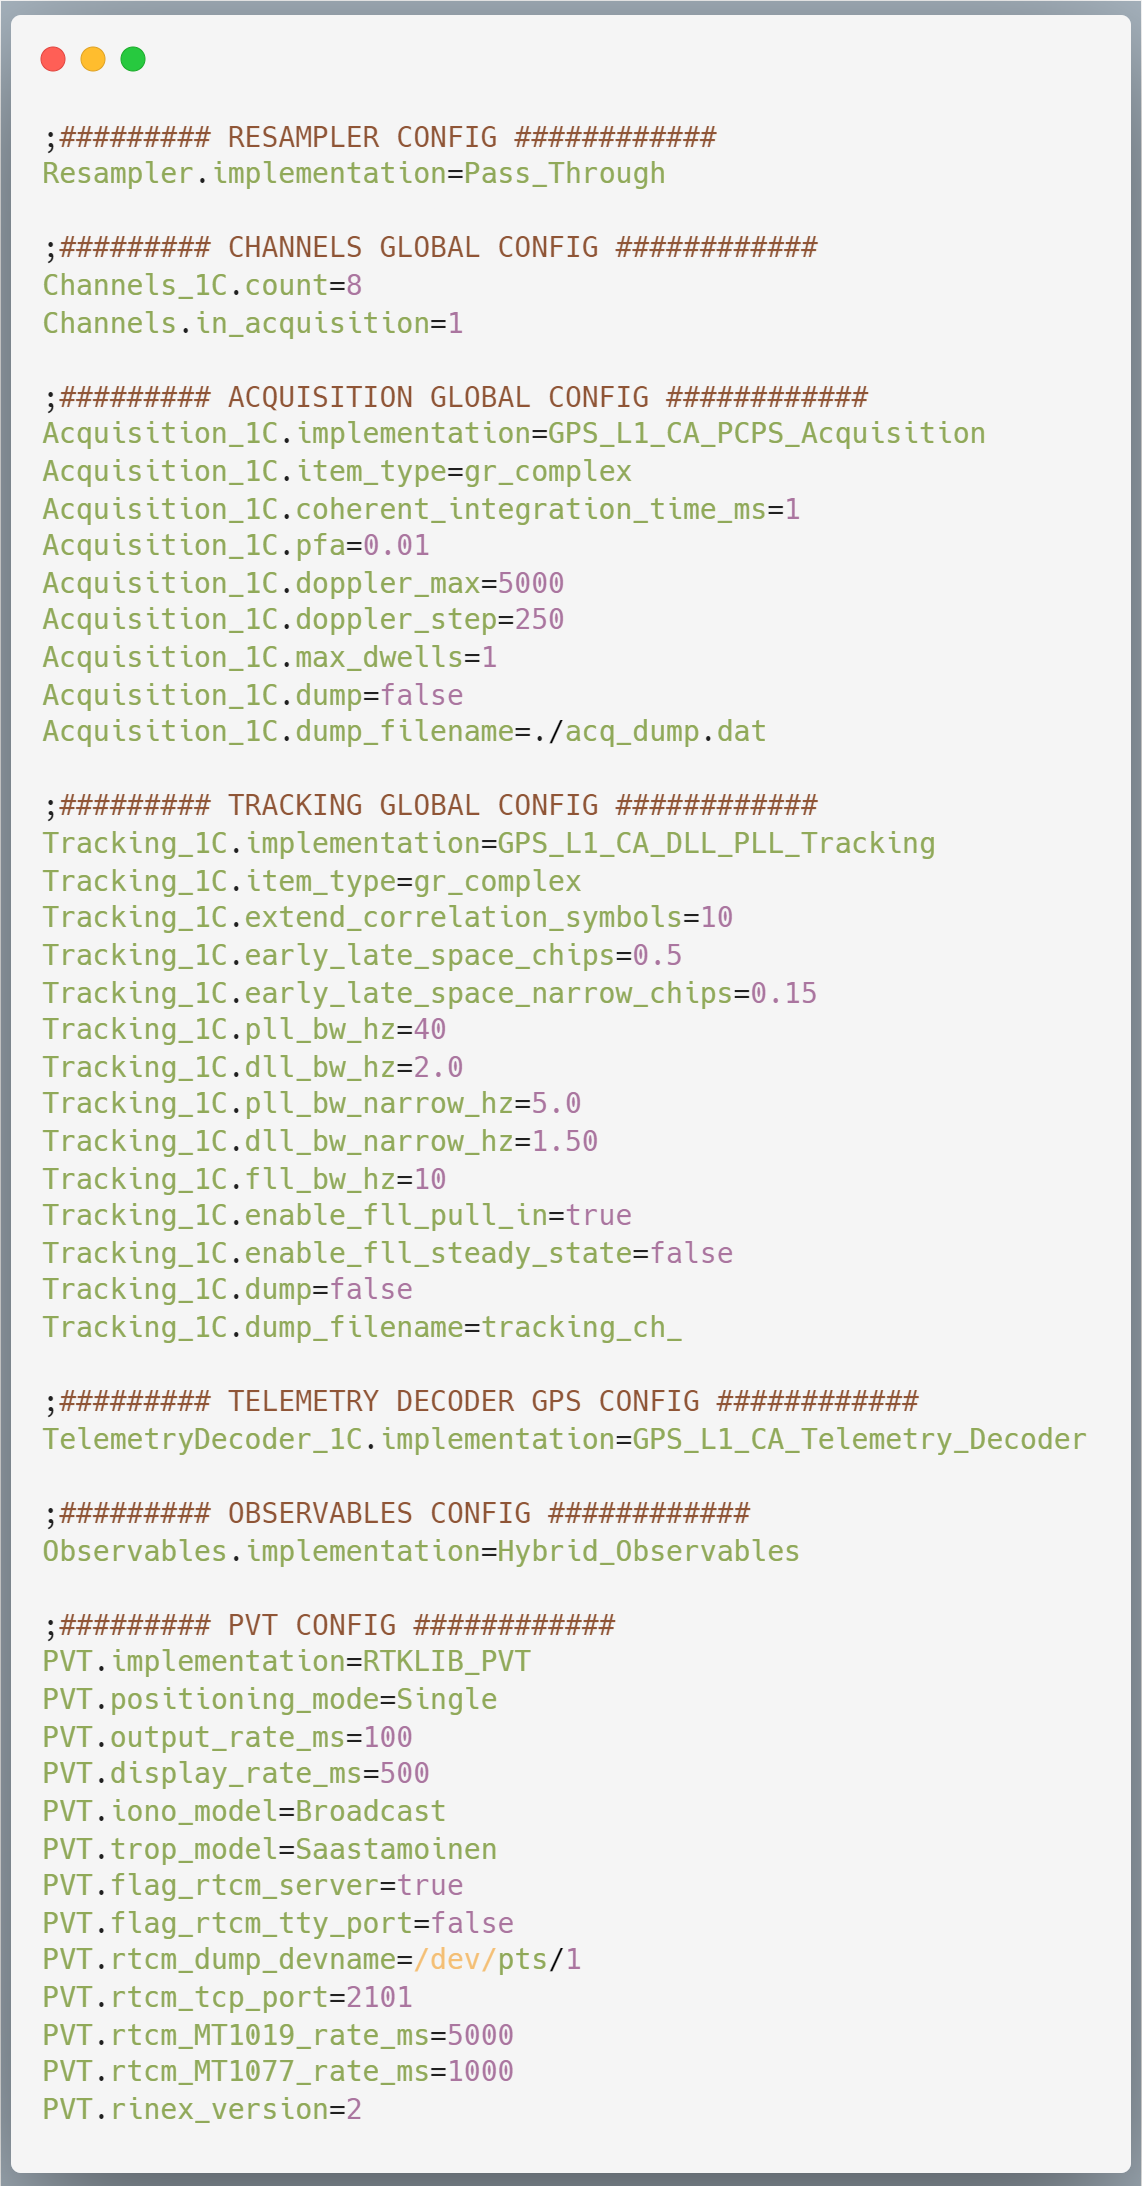
\includegraphics[width=0.6\linewidth]{sdr_front2.png}
\end{center}


\chapter*{appendix 3}
\addcontentsline{toc}{chapter}{appendix 3}
\begin{center}
	\url{https://github.com/ThePurpleOne/gnss_spoofing}
\end{center}



%%% COMMENT THESES LINES IF YOU DO NOT USE DEDICATED TOC FOR appendixS
\stopcontents[annexes]
\resumecontents[default]
%%% /COMMENT THESES LINES IF YOU DO NOT USE DEDICATED TOC FOR appendixS